\documentclass[a4paper,twoside,10pt]{report}
%picture imports
\usepackage{graphicx}
\usepackage{color}
 \usepackage{fancyhdr}
\definecolor{lbcolor}{rgb}{0.85,0.85,0.85}

%sourcecode formatting
\usepackage[final]{listings}
\usepackage{url}


\lstloadlanguages{Eiffel,bash,Java}
\newcommand{\eiffellisting}{\lstset{basicstyle=\small,language=Eiffel,tabsize=2,backgroundcolor=\color{lbcolor},frame=tb,breaklines=true}}
\newcommand{\bashlisting}{\lstset{basicstyle=\small\tt,language=bash,tabsize=2,backgroundcolor=\color{lbcolor},frame=tb,breaklines=true,morekeywords={svn,geant,mkdir,activate_estudio}}}
\newcommand{\javalisting}{\lstset{basicstyle=\small,language=Java,tabsize=2,backgroundcolor=\color{lbcolor},frame=tb,breaklines=true}}
\newcommand{\identifier}[1]{\texttt{#1}}
\newcommand{\figref}[1]{Figure \ref{#1}}
\newcommand {\class}[1] {\texttt{#1}}
\pagenumbering{roman}

\begin{document}

%opening
\title{Selective Capture and Replay for Eiffel}
\author{Stefan Sieber}

\begin{titlepage}
	\begin{flushleft}
		\includegraphics[width=100pt]{illustrations/SE.png}
	\end{flushleft}

	\vskip 50pt
	\begin{center}
		\Huge \textbf{Capture and Replay for Eiffel}
	\end{center}

	\vskip 100pt
	\begin{flushright}
		\large \textbf{Stefan Sieber}\\
		\vskip 10pt
		02-911-790\\
		Master Thesis\\
		Summer 2007\\
	\end{flushright}
	
	\vskip 20pt
	\begin{flushright}
		\large Chair of Software Engineering\\
		Department of Computer Science\\
		ETH Z\"{u}rich
	\end{flushright}
		
	\vskip 20pt
	\begin{flushright}
		\large Andreas Leitner\\
		Prof. Bertrand Meyer
	\end{flushright}

	\vskip 50pt
	\begin{tabular*}{1.00\textwidth}{@{\extracolsep{\fill}}lr}
		 \includegraphics[width=100pt]{illustrations/ETH.png} &
		 \includegraphics[width=100pt]{illustrations/INF.png}
	\end{tabular*}
	\vfil
\end{titlepage}

%prolog
\addtolength{\parskip}{0.5\baselineskip} % add extra spacing between paragraphs
\newpage
\pagenumbering{roman}
\include{abstract}

% table of contents
\addtolength{\parskip}{-0.5\baselineskip} % reset paragraph spacing
\tableofcontents

\newpage

% chapters
\pagenumbering{arabic}
%configure headers:
%XXX reenable fancyhdr, when fancyhdr.sty was found.
% \pagestyle{fancy}%
% \renewcommand{\headrulewidth}{0.3pt}
% \renewcommand{\footrulewidth}{0pt}
% \renewcommand{\chaptermark}[1]{\markboth{\MakeUppercase{#1}}{}}
% \renewcommand{\sectionmark}[1]{\markright{\MakeUppercase{#1}}{}}
% \fancyhf{}
% \fancyhead[LE,RO]{\thepage}
% \fancyhead[LO]{\rightmark}
% \fancyhead[RE]{\leftmark}
% \fancyfoot{}

\addtolength{\parskip}{0.5\baselineskip} % add extra spacing between paragraphs
\chapter{Introduction}
%The initial part of the introduction was taken from the abstract. Maybe some modifications are to be done here...
Debugging applications is very tedious work. One of the hardest steps to find a fault in a program is to reproduce the steps that lead to the associated program failure. Capture and replay aims at simplifying this process. In order to be able to replay an application, it is necessary to isolate the deterministic part of the application that needs to be replayed (observed part) and the non-deterministic parts, like user input, storage or network (unobserved part). Once the behavior of the unobserved part can be captured and replayed, it is also possible to replay the observed part. Although capture and replay is commonly known as capturing mouse and keyboard events, there are approaches that go further and capture events from all interactions with the environment. All these approaches have one thing in common: They have a fixed border between observed and unobserved part.

Selective Capture and Replay \cite{orso05may} makes it possible to individually define the observed part, thus it offers the possibility to optimize the amount of information that needs to be captured. To reduce the amount of captured data, Selective Capture and Replay uses another amazingly simple technique: Whenever an object passes the border, only its type and a unique identifier is recorded, unless the passed object is from a basic type. This is sufficient to allow a complete replay, because the notion of observed and unobserved part is extended from code to objects. If an observed object was passed, the object will be correctly rebuilt during replay, thus it is not necessary to store any additional information. If the passed object is not observed, it is only a stub anyway and all accesses to it will result in events that can be replayed. Therefore the recorded data will be linear to the number of variables passed through the border, in contrast to other techniques which capture the whole data that is passed.

These advantages make Selective Capture and Replay an interesting approach to implement capture and replay for Eiffel. It would allow capture and replay functionality for whole applications with some changes in the runtime and modifications in the libraries that are significantly smaller than traditional approaches.

The original implementation for Selective Capture and Replay was made for Java. The technique proposed in the original paper can not be completely applied to Eiffel because some language features differ between Eiffel and Java. Some of these differences make an implementation easier (e.g. it is not possible to change attributes of other classes) and some make it harder (e.g. multiple inheritance). Selective Capture and Replay heavily relies on code instrumentation to capture accesses across the border. The original implementation instruments method and attribute accesses on the caller (client) side, which is not possible for Eiffel: Due to multiple inheritance, it cannot be determined whether the callee (server) is observed or not. Therefore we instrument code at the callee side. Another modification that was made to the instrumentation allows switching between capture and replay without recompilation. Although this feature costs in terms of performance, it is necessary for Eiffel, because reinstrumenting the code would require a complete recompile. The original implementation allows faster instrumentation, as it instruments at the bytecode level and therefore doesn't need a complete recompile when the code should be instrumented differently.

When speaking about performance, it is important to note that the current implementation was not optimized for speed. It was more important to provide a running implementation that shows whether Selective Capture and Replay is applicable for Eiffel. Nonetheless, some performance measurements will be presented, based on a simple example application.




\chapter{Related Work}
\section{Overview}
Because replaying application runs is important in order to be able to debug or test applications, there exist many techniques that implement capture and replay. As mentioned before, one of the basic steps in order to be able to capture and replay an application is to distinct between the deterministic core (the \emph{observed part}) and the non-deterministic environment (the \emph{unobserved part}) of the application like user input, network or external storage.

In general, capture and replay can be divided into two phases: The \emph{capture phase}, where the application is run and the information that is needed for replaying the application is captured and the \emph{replay phase} where the application is replayed based on this information.

During \emph{capture phase}, the capture and replay implementation needs to record the information that will later be needed to replay the observed part. In general this is at least all information that is passed from the unobserved part to the observed part. The information is captured by some management code that was introduced by the capture and replay framework (\figref{fig:GenericCrStructure_capture}).
\begin{figure}[h]
  \centering
  \includegraphics[width=0.5\textwidth]{illustrations/capture_and_replay_generic_structure_capture}
  \caption{Generic structure of a capture and replay technique - capture phase}
  \label{fig:GenericCrStructure_capture}
%\includegraphics{illustrations/capture_and_replay_generic_structure}
\end{figure}

During \emph{replay phase} the management code needs to replace the unobserved part ( 
\figref{fig:GenericCrStructure_replay}) in order to replay the run of the observed part. Depending on the part of the application that was defined to be unobserved, the management part can act both as a driver (e.g. in the case of mouse events) and stub (e.g. in the case of a network socket). 
%Schema dazu: Capture phase & Replay phase , observed & unobserved part && log
\begin{figure}[h]
  \centering
  \includegraphics[width=0.4\textwidth]{illustrations/capture_and_replay_generic_structure_replay}
  \caption{Generic structure of a capture and replay technique - replay phase}
  \label{fig:GenericCrStructure_replay}
%\includegraphics{illustrations/capture_and_replay_generic_structure}
\end{figure}

Different implementations make different assumptions about what behaves the same (is deterministic) and what changes its behaviour throughout different runs of the application. Therefore they define different portions of the program as observed and unobserved part. Here we will categorize the different implementation based on what is defined to be unobserved.

\section {Capturing User Input}
The best known capture and replay technique is used for GUI testing. Here, keyboard and mouse events are considered to belong to the unobserved part. The exact location where these events are captured may vary (inside the application or through the operating system), but the advantages and limitations mostly stay the same. Usually, capture and replay of user input is used for regression testing. In that setup, the tester executes a sequence of actions on the applications GUI while capturing is enabled. These recorded actions can be replayed on the application in order to check if there were regressions. Abbot \cite{abbot} is an example of such a tool, although it offers more features than only capture and replay of user interactions.
\subsection{Advantages}
This technique is easy to understand, because it is based on a simple abstraction.
\subsection{Limitations}
If this technique is implemented in a very naive way (i.e. only capturing the location of mouse events, not the targets), a changed GUI layout renders a recorded run unusable. This is especially painful, if the capture and replay is used for regression tests. Another problem is that most applications use more than just the GUI to interact with their environment. As soon as the application uses the file system or the network, too, it is necessary to make sure, that the behaviour of this environment is the same every time the program is replayed. Otherwise the assumption, that the observed space behaves deterministically would be broken, which results in an incorrect replay of the application.

\section {Capturing Interactions with the Libraries}
JRapture \cite{jrapture} uses an approach that has the potential of replaying more complex applications. JRapture is a tool for capturing and replaying Java applications in the field. In addition to capturing and replaying, it also offers a profiling interface that permits the program to be instrumented for profiling in the replay phase.

In our model of capture and replay techniques, JRapture draws the border between observed and unobserved part between the Java API and the core of the program. They achieve this by instrumenting the Java API classes. JRapture supports multithreaded applications, but it does not guarantee a deterministic replay of concurrent applications.

\subsection{Advantages}
JRapture has the potential to replay more complex applications that involve file and network access. In principle it is able to replay every interaction of the observed part with its environment as long as these interactions are executed through the Java API.
\subsection{Limitations}
JRapture relies on a modifed version of the Java API, which was created by manual instrumentation of it. Only a subset of the Java API is covered by this instrumentation yet, for example it lacks support for network I/O at the moment. Thus although JRaptures approach has the potential of replaying complex applications, it does not succeed yet to do so. Another drawback of the manual instrumentation is that applications that interact with the environment through other mechanisms than the Java API (for example through the Java Native Interface JNI) can not be supported without additional manual instrumentations.
%\section {Capturing Interactions with the Operating System}
%Operating System - Library
%TODO: gehoert bugnet hier auch rein???
%state (wird das als cr bezeichnet?) vs. events
\section {Capturing Interactions with the Scheduler}
The techniques presented so far did not consider thread scheduling as another source of non-determinism. DejaVu \cite{dejavu}, a capture and replay tool for Java, considers thread scheduling as its only source of non-determinism, thus thread scheduling belongs to its unobserved part. Because threads are often scheduled by the operating system, it is not easy to instrument the scheduler in order to detect thread switches. DejaVu therefore introduces the concept of \emph{logical thread schedule} which is a simplified version of the real thread schedule (the \emph{physical thread schedule}). The \emph{logical thread schedule} contains enough thread schedule information to reproduce the execution behaviour of the program under the assumption that the thread schedule is the only source of non-determinism. By detecting some critical events during capture phase such as access to shared variables, and synchronization events, DejaVu is able to deduce this logical thread schedule.

%XXX Rettet der 2. Satz unser Modell????
DejaVu does not completely fit into our generic schema of a capture and replay technique from the implementation point of view, because the information passed between unobserved part (scheduler) and observed part (the application) is not directly captured but a simplified version is deduced. However, the semantic stays the same because the part of information that matters to the application is captured and can be used to replay the program afterwards.

\subsection{Advantages}
DejaVu succeeds in capturing and replaying a concurrent application that does not use any other source of non-determinism than the thread scheduler. Of the techniques listed here, DejaVu is the only one that takes thread scheduling into account.
\subsection{Limitations}
Because DejaVu only focuses on thread scheduling as a source of non-determinism of a program, it is not suited for capturing and replaying a general program. Nevertheless the technique of DejaVu could be combined with another capture and replay technique in order to build a system that allows deterministic replays of general multithreaded programs.

\section{Selective Capture Replay}
The capture and replay techniques seen so far all define a border between observed and unobserved part. In contrast to these techniques, \emph{Selective Capture and Replay} \cite{orso05may} implemented for java, offers the user the possibility to make its own definition of observed and unobserved part of the system. Observed and unobserved part are both defined as a set of classes. The interactions between observed and unobserved part are captured using automated code instrumentation.
\subsection{Advantages}
The main advantage of this technique is its flexibility. The possibility to individually define observed and unobserved part makes it possible to minimize the amount of data that is exchanged between these two parts by a smart choice of the border. Because no custom capture mechanism is needed, applications that use own libraries to interact with the non-deterministic environment can be supported without manual instrumentation. 
\subsection{Limitations}
Although Selective Capture and Replay is a very generic approach, it assumes that multithreading does not cause non-deterministic behaviour of the observed part. Thus it is not generally possible to replay a program run that involves data races.
%Wir beachten call durations nicht (!)

%Überblick über das Paper
%Limitations (polymorphism / dynamic binding) --> oder doch nicht? she. Annahme über observed set.
%Benefit for cdd


\chapter{Preleminaries}
\section{Example Application}
This example application will be used repeatedly in this report. By explaining the application in detail here, the explanations that use it should be clearer to the reader.

Imagine a Bank that manages different bank accounts which can be identified by their name. Customers can deposit and withdraw money from their accounts by using ATMs. The customers interact with the ATM through some kind of user interface. This user interface will be implemented in different ways (textual or graphical), depending on our use case (\figref{fig:example_class_diagram}). All operations on the bank account will be dispatched from the ATM to the bank. 

To make the example more interesting, we will some times assume that BANK accesses the network, file system and a database. This will make capture and replay of the system more difficult. %TODO: wahrscheinlich sollten wir das ins Klassen-diagramm nehmen?
%TODO: anmerken, dass die Klassen und methodennamen an Eiffel Styleguide angepasst sind, aber die gleichen Namen auch fuer die Java Beispiele verwendet werden.

 \begin{figure}[ht]
   \centering
   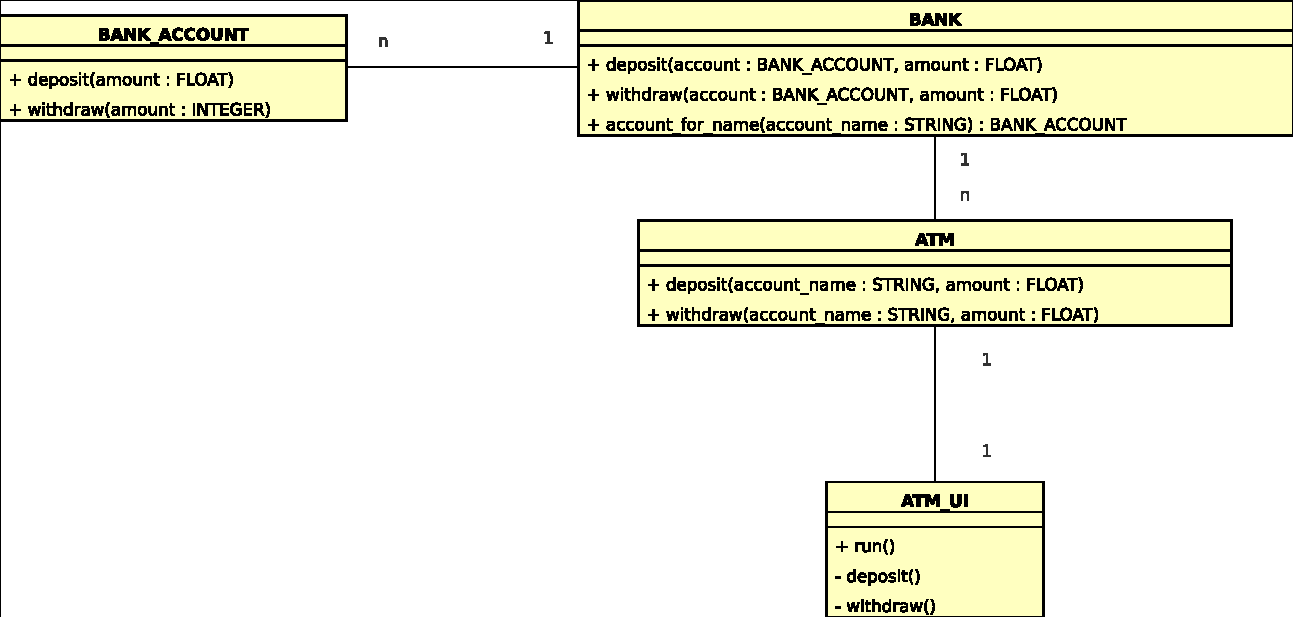
\includegraphics[width=1\textwidth]{illustrations/example_class_diagram}
   \caption{Class Diagram of the Example}
   \label{fig:example_withdraw_sequence}
 %\includegraphics{illustrations/capture_and_replay_generic_structure}
\end{figure}

One use case is money withdrawal by a customer via an ATM. The customer launches the withdrawal operation on the ATM\_UI. The request is passed through the ATM to the BANK which then withdraws the money from the Account. The sequence diagram (\figref{fig:example_withdraw_sequence}) should clarify how the classes interact with each other.

\begin{figure}[ht]
   \centering
   \includegraphics[width=1\textwidth]{illustrations/example_withdrawal}
   \caption{Withdrawal Operation Invoked by the User}
   \label{fig:example_class_diagram}
 %\includegraphics{illustrations/capture_and_replay_generic_structure}
\end{figure}

\section{Selective Capture and Replay}
After giving the overview about the different capture and replay techniques, our choice will be described here in detail. This chapter summarizes papers from Joshi and Orso about the Java implementation of selective capture and replay (SCARPE) \cite{orso05may, orso06}.

\subsection{Technique and Terminology}
\begin{figure}[ht]
  \centering
  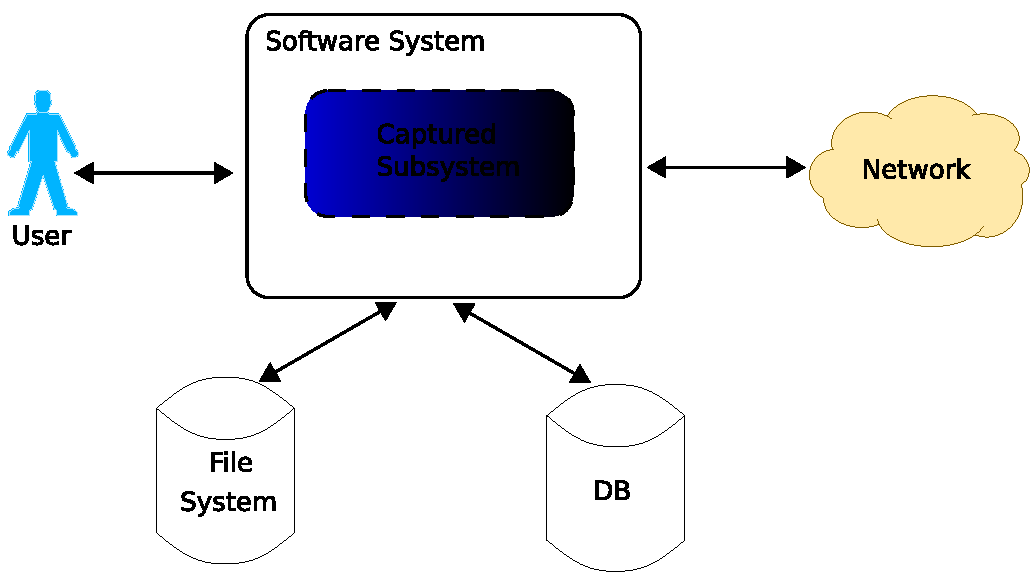
\includegraphics[width=1\textwidth]{illustrations/scr_overall_schema}
  \caption{System Layout of the Example Application (derived from \cite{orso05may})}
  \label{fig:scr_overall_schema}
%\includegraphics{illustrations/capture_and_replay_generic_structure}
\end{figure}
This technique lets the user choose the subset of the program that should be captured and replayed (\emph{captured subsystem}, \figref{fig:scr_overall_schema}). It then only captures the execution data of that subsystem, ignoring the other parts of the system. The relevant interactions between the captured subsystem and the outside world is captured in terms of events; those events are read during the replay phase in order to replay the corresponding interactions. Only the essential part of the information that traverses the border between the captured subsystem and the rest of the system is captured. This is a significant improvement over other existing techniques that capture all the data, especially when big datastructures are passed over the border and only a part of those datastructures is actually accessed.

Here are some terms that are used to describe selective capture and replay:
\begin{description}
	\item [The observed set] is the subsystem that was selected for capture and replay.
	\item [The observed classes] are the classes in the observed set. Observed code is defined analogous.
	\item [Observed methods and fields] are the fields and methods of the observed classes.
\end{description}
\emph{Unobserved set},  \emph{unobserved classes}, \emph{unobserved code}, \emph{unobserved methods} and \emph{unobserved fields} are the analogous terms for the part of the system that was not selected for capture and replay.
\begin{description}
	\item [External code] denotes unobserved and library code together.
	\item [Unmodifiable classes] are the classes whose code can not be modified (e.g. some system classes such as \texttt{java.lang.Class}) due to constraints from the Java Virtual Machines
	\item [Modifiable classes] are all classes except the \emph{unmodifiable classes}
\end{description}

The technique is divided in two main phases: capture and replay. \figref{fig:scr_capture_replay_phase} illustrates the setup of of these two phases in selective capture and replay.
\begin{figure}[ht]
  \centering
  \includegraphics[width=0.8\textwidth]{illustrations/scr_capture_replay_phase}
  \caption{Capture and Replay Phase in Selective Capture and Replay}
  \label{fig:scr_capture_replay_phase}
%\includegraphics{illustrations/capture_and_replay_generic_structure}
\end{figure}
The \emph {capture phase} takes place when the application is run for recording. Before the application starts, the boundaries of the observed set are identified and the application is instrumented in order to be able to capture interactions between the observed set and the rest of the system. While the application runs, the instrumentation generates the events for these interactions and writes them to the \emph{event log}.

In the \emph{replay phase}, the technique generates the \emph{replay scaffolding}. The replay scaffolding uses the event log to replay the events on the observed set. Replaying consists both of performing actions on the observed set (e.g. invocation of a method of the observed set) and consuming actions of the observed set (e.g. receiving a method invocation originally targeted to the unobserved set), thus the replay scaffolding acts both as a driver and stub.

\subsection{Capture Phase}
%Capture Phase
\subsubsection{Capturing Partial Information}
The technique for capturing only partial information instead of the whole data that flows into unobserved set relies on \emph{object IDs}. An object ID uniquely identifies a class instance. SCARPE introduces the object ID into the program by adding an additional field to all modifiable classes. It further instruments the creation constructors of these classes so that the unique object ID is acquired from a global counter. For unmodifiable classes however, a reference map is needed to store the object ID of its instances. The object ID for instances of unmodifiable classes is acquired when it is looked up the first time. The reference map uses weak refences so that the referenced objects can be collected by the garbage collector to avoid memory leaks.

Instead of recursively serializing the data that crosses the boundaries of the observed set, selective capture and replay only records a small part:
\begin{itemize}
 \item Scalar values (values of a basic type) are fully captured.
 \item For Objects, the technique only captures the object ID and the type. The type is used to restore the object again during replay phase.
\end{itemize}

To see the advantages of this approach clearer, consider the case when \class{BANK} tries to find out the time of the last log entry of an \class{ATM}. Assume that the classes \class{BANK} and \class{BANK\_ACCOUNT} belong to the observed set and the rest of the application belongs to the unobserved set. The following instructions access the atm's log and print the time of the last log entry:
\javalisting
\begin{lstlisting}
 ATM_LOG log = atm.log
 print (log.time_of_last_entry)
\end{lstlisting}
\class{ATM\_LOG} could contain a thousand of log entries. In a traditional approach, due to the access to the log, the whole data structure including all log entries would be serialized each time the log is accessed. With the approach of selective capture and replay, only the log's object ID and type is written to the event log, as well as another method call to an unobserved class due to the call to time\_of\_last\_entry. This reduces the size of the event log significantly, because only the the data that is used needs to be written down.

Although this powerful approach is amazingly simple, it is not always easy to grasp. Here is a short reasoning why it works:
\begin{enumerate}
  \item [1)] Instances of observed classes are fully populated during replay, because all actions from the unobserved set are replayed on them and the actions from the observed set are executed on them as in the original run.
  \item [2)] During replay, observed code accesses to methods or fields can either return instances of observed classes or instances of unobserved classes.
  \item [3)] When an object of an observed class is returned, it is fully populated due to 1) and therefore its fields and methods can safely be accessed.
  \item [4)] When an object of an unobserved class is returned, each further access to a field or method from observed code to that object would result in the capturing of another boundary crossing event. Therefore the results of these accesses can be reconstructed during replay.
  \item [5)] Therefore, it is assured that during replay, it is possible for the observed code to access the fields and methods like it did in the original run.
\end{enumerate}



\subsubsection {Interactions between Observed and External Code}
Method calls are an elementary way to communicate between observed and external part of the application. The technique captures calls in both directions: from observed to unobserved code and vice versa. The events related to method calls that are captured are:

\begin{description}
 \item  [OUTCALL] events that represent calls from observed code to unobserved methods.
 \item [INCALL] events that represent calls from unobserved code to observed methods.
 \item [OUTCALLRET] events for the return from outcalls
 \item [INCALLRET] events for the return from incalls
\end{description}

OUTCALL and INCALL events (\emph {call events})  have the same attributes:

\begin{description}
 \item [Receiver] The receiver object
 \item [Method called] Signature of the called method.
 \item [Parameters] The list of scalar values and objects passed to the method.
\end{description}

Capturing of call events involves capturing of scalar values and objects. They are written to the log as follows:

\begin{description}
 \item [Scalar values] are fully written to the log.
 \item [Objects] are written by storing their type and object ID. For null values, the object ID is set to zero. 
\end{description}

OUTCALLRET and INCALLRET events (\emph{callret events}) have only one attribute: the returned value.

OUTCALL and OUTCALLRET events are captured by instrumenting the observed code. A probe is added to all calls to external methods. It is not always possible to distinguish calls to observed code from calls to unobserved code, as we will discuss later.

To capture INCALL and INCALLRET events, proxy methods are introduced in a way that makes it unnecessary to instrument external code. It is ensured that calls inside the observed code don't call these proxy methods but the actual methods. Thus calls from observed code to observed methods can be executed without overhead.

Field Accesses are another source of interaction between observed and external classes. Read accesses from unobserved to observed code don't influence the execution behaviour of the observed code therefore they are not captured. Thus three kinds of events are recorded:

\begin{description}
 \item [OUTREAD] events are generated when observed code reads the content of an unobserved field.
 \item [OUTWRITE] events denote write accesses from observed code to unobserved code.
 \item [INWRITE] events are write accesses from unobserved code to observed code.
\end{description}

OUTREAD, OUTWRITE and INWRITE have the same attributes:

\begin{description}
 \item [Receiver:] The object whose field is accessed.
 \item [Field Name:] The name of the field that is accessed.
 \item [Value:] The read or written value.
\end{description}

OUTREAD and OUTWRITE events are captured by adding probes in the observed code where fields of external classes are accessed. INWRITE events are captured in the same way, but here the unobserved code is instrumented whenever an observed field is written. Here, the same problem as with OUTCALL events arises: It is not always possible to determine whether an observed or unobserved field is accessed.

Exceptions are another interaction mechanism that needs to be considered for capture and replay. Because exceptions were not implemented in our Eiffel implementation of selective capture and replay, they will be treated only briefly. For Exceptions, to more types of events were introduced:
\begin{description}
 \item [EXCIN] events are for exceptions that propagate from the external to the observed code.
 \item [EXCOUT] events are for exceptions that propagate from the internal to the external code.
\end{description}
EXCOUT events are captured by wrapping all observed methods with a \texttt{try-catch} block. By wrapping instructions that call an observed method with an exception handler,  EXCIN events are captured.

\subsection{Replay Phase}
During the replay phase, the observed code is reexecuted based on the event log that was gathered during the capture phase. Before replaying the observed code, selective capture and replay instruments the code based on the interactions between observed and external code. 

\subsubsection{Object Creation}
In the replay phase, object IDs are treated in a different way. Now it is necessary to find the object that matches a given object ID, not reverse. In order to allow this resolving, the technique uses a reference map that maps the object ID to all available  objects. The technique extracts the object IDs from the event's attributes and then retrieves the associated object or creates it. How these objects are created depends on whether they are instances of observed or external classes.
\begin{description}
 \item [Instances of External Classes:] For external classes, \emph{placeholder objects} are created. These objects have the correct type in order to support reflection in the observed code, but their state is irrelevant. After creation, the objects are registered in the reference map.  %placeholder constructors are not that important for us --> no need to describe them...
 \item [Instances of Observed Classes:] Instances of observed objects are either created automatically by the observed code or there must be an INCALL event to the constructor in the event log. When replaying an INCALL to a constructor, an entry for the object is added to the reference map.
 \item [Null Values] If the object ID is zero, \texttt{null} is returned.
\end{description}

%---
\subsubsection{Events Replaying}
For the replay phase, a scaffolding is generated that imitates the behaviour of the external code, thus behaves both as a driver and stub. Whenever control returns to the scaffolding, it checks whether the received event matches the next event in the log. If the events don't match (\emph{out-of-sync events}), a message is displayed to the user, who can chose whether to ignore the discrepacy and continue, or stop the replay.  Out-of-sync events can only occur, if the code was changed between capture and replay phase, for example because the technique is used for regression testing. If the events from log and replay match, the event in the log is  consumed and replay continues.

In contrast to INCALL, INWRITE, OUTREAD, OUTCALLRET and EXCIN, which are necessary to replay the observed code correctly, OUTCALL, INCALLRET, OUTWRITE, EXCOUT are not necessary to replay the observed code, but they can be used as oracles for regression testing. %XXX is this really correct??? I can't imagine that they can guess the object ID's without these events!!!

\begin{description}
 \item [INCALL Events] To replay INCALL events, the method first retrieves the target object from the reference map. If the target object is not in the reference map, it must be either a call to a constructor or a static call. Then, it retrieves the parameters from the reference map, or creates the scalar values corresponding to the parameters. If the object can't be retrieved from the reference map, a placeholder object is created. Then, the technique can call the specified method with all arguments; the control flows to the observed code. 
 \item [INCALLRET Events] INCALLRET events are not essential for replaying the observed code. They occur as a result of INCALL events and are consumed by the replay scaffolding. To ensure a correct replay, the scaffolding checks if returned value conforms to the one of the next event in the event log.
 \item [OUTCALL Events] All invocations to unobserved methods from the observed code are replaced by two instructions: (1) The call to a special feature in the scaffolding (\texttt{consumeCall}) and (2) The assignment of the result of the invocation. For example \texttt{TIME t = atm\_log.time\_of\_last\_entry()}, with TIME and ATM\_LOG both being in the package \texttt{foo}, would be replaced by the following instructions:
\begin{lstlisting}
 Object tmp = scaffolding.consumeCall("foo/ATM_LOG",
                /*object ID for atm_log*/,
                "time:()Lfoo/TIME",
                /*empty array of parameters*/);
 TIME t = (TIME) tmp;
\end{lstlisting}
The scaffolding checks whether type, parameters, target and methodname of the next event from the log matches to the reported call. If everything is allright, then replay continues with the next event, otherwise an error is reported to the user.
 \item [OUTCALLRET Events]As these events occur as a result of OUTCALL events, they are treated within \texttt{consumeCall}. The method looks up the return value in the event log and retrieves it using the reference map. 
 \item [OUTREAD and OUTWRITE Events] To replay these events, accesses to unobserved fields are instrumented in the observed code, by calling associated methods from the scaffolding, \texttt{consumeRead} for OUTREAD events and \texttt{consumeWrite} for OUTWRITE events. For example the instruction \texttt{ATM\_LOG = atm.log}, with ATM\_LOG and ATM both belonging to package \texttt{foo}, would be replaced by the following instruction:
\begin{lstlisting}
 ATM_LOG log = scaffolding.consumeRead ("foo/ATM",
                /*Object ID for atm*/,
                "val")
\end{lstlisting}
The methods \texttt{consumeRead} and \texttt{consumeWrite} check if the event from the log matches the detected one. The method \texttt{outRead} furthermore returns value associated with the event.
 \item [INWRITE Events] In order to replay an INWRITE event, the scaffolding retrieves the target, the name of the field that should be modified and the value to be assigned. It resolves the target, which must exist unless it is a static field access. The value to be assigned is resolved as well or created if it does not exist yet. Finally the scaffolding sets the field of the target to the specified value.
 \item [EXCIN and EXCOUT Events]  To replay EXCIN events, the method \texttt{consumeCall} creates and throws a corresponding exception. This is possible, because EXCIN events can only occur during an outcall. EXCOUT events, which are generated by the observed code, are caught by the replay scaffolding and compared to the next event in the event log. If the exception matches the event from the event log, replay continues.
\end{description}

\subsubsection{Assumptions}
Selective capture and replay works under some assumptions:
\begin{itemize}
 \item It is assumed that there is no direct access from unmodifiable classes to fields of observed classes.
 \item Because native code is not instrumented, they also assume that there is no direct access from native code to observed fields.
 \item The technique can not guarantee the same thread schedule during capture and replay phase. Therefore it is assumed that the interleaving due to multi-threading does not change the behaviour of the observed code.
 \item They assume that runtime exceptions occur deterministically. This is necessary, because exceptions generated in the observed code are consumed, but not replayed.
\end{itemize}

\subsubsection{Special Cases}
\begin{description}
 \item [Polymorphism and Dynamic Binding] It is not always possible to determine whether an event is internal or external, when it depends on the dynamic type of the receiver. In these cases, it is necessary to add a runtime check to determine whether the receiver is an internal or external class, which is done using the \texttt{instanceof} operator. \texttt{XXX Is this insertion here valid?} We assume that this case occurs at least in examples that use multiple interface inheritance, where it can not be assumed that the implementors of an interface are either all in the observed set or all in the unobserved set.
 \item [Inheritance] If a class \emph{c} is in the observed set, but not all of \emph{c's} subclasses, creating an instance of any of \emph{c's} subclasses would result in the creation of an instance of \emph{c}. To avoid this issue, it is required that if a class \emph{c} is added to the observed set, all subclasses of \emph{c} are also in the observed set. We assume that the side effect described here is an implementation specific problem, and could be avoided.
 \item [Reflection] The technique handles most cases of reflection, however in some cases, additional instrumentation is required (e.g. if reflection is used in external code to modify fields of observed classes). 
 \item [Access Modifiers] In order to replay recorded executions, in some cases it is necessary to change access modifiers. We assume that this applies primarily to the \texttt{protected} modifier, which may prohibit access to observed classes from within the replay scaffolding.
 \item [Garbage Collection] To allow the collection of unused objects, the technique must make sure that it does not keep references to unused objects. For example the reference map must use weak references to avoid memory leaks.
 \item [Finalize] Calls to \texttt{finalize} are non-deterministic in Java, thus they can generate out-of-sync events during the replay phase. Therefore calls to \texttt{finalize} are treated in a special way: when receiving a call to \texttt{finalize}, the technique consumes the next matching entry in the event log, that is a call to \texttt{finalize}.
\end{description}

%Polymorphism and Dynamic Binding
%Inheritance
%Reflection
%Access Modifiers
%Garbage Collection
%Finalize
%-Eiffel compilation model (?)
%-CDD (?)
\chapter{Capture and Replay for Eiffel}
\section{Relevant Differences between Eiffel and Java}
\section{Differences in the Requirements}
\section{Idea for Code Instrumentation}


%weitere Unterschiede:
% - creation procedures nicht gesondert instrumentiert --> synchronisierung bei outcalls. sonst muessten die unobserved Klassen nicht instrumentiert werden (nur outcallret) (?)

\section {Limitations}
%-Konstruktoren nach ANY exportiert (fehlende unterstuetzung von Eiffel-Seite fuer Konstruktoren)
%- Access modifiers e.g. export of a observed feature only to an unobserved class --> replay not possible.

\chapter{Experimental Results}
\section{Example Application}
\section{Results}
\section{Conclusion}
%Eiffel Vision Beispiel, mit unterschiedlichen observed sets

\chapter{Future Work}
%Fehlende C/R und Language Features beschreiben, sowie einen möglichen Lösungsansatz.
\chapter{Appendix}

\subsection{Log File Grammar}

log ::= event* \\
event ::= call $\mid$ return $\mid$ outread\\
call ::= calltype entity methodname entity* \texttt{“\%N”} \\
return ::= returntype [entity]  \texttt{“\%N”}\\
outread ::= \texttt{OUTREAD} entity attribute\_name entity
calltype ::= \texttt{INCALL} $\mid$ \texttt{OUTCALL} \\
returntype ::= \texttt{INCALLRET} $\mid$ \texttt{OUTCALLRET} \\
methodname ::= identifier \\
attribute\_name ::= identifier \\
entity ::= (object $\mid$ value) \\
size ::= integer \\
object ::= \texttt{[NON$\_$BASIC} typename object\_id \texttt{]} \\
value ::= \texttt{[BASIC} typename \texttt{"} string \texttt{"]} \\
typename ::= identifier \\
object\_id ::= integer\\
identifier ::= [A-Za-z]character*\\
string ::= character*\\

\subsection{capture-phase performance measurements}
\begin{itemize}
	\item normal application: 2.5s
	\item Captured application: 30s
	\begin{itemize}
		\item RECORDER: 1.7s\\
		\item SERIALIZER: 26s
		\begin{itemize}
			\item write$\_$statements: 16s
			\begin{itemize}
				\item file.put$\_$string: 4s
				\item object$\_$id: 7s
				\item other: 5s
			\end{itemize}
			\item is$\_$basic$\_$type: 3s
			\item other: 7s
		\end{itemize}
	\end{itemize}
\end{itemize}

\bibliographystyle{plain} 
\bibliography{thesis}

\end{document}


